\chapter{Wprowadzenie i instrukcja użytkowania systemu kontroli wersji Git}
\label{ap:1}

\section{Wprowadzenie}

Do wspomagania równoległego, rozgałęzionego procesu rozwoju projektu przez wielu programistów zdecydowano się wykorzystać rozproszony system kontroli wersji Git. 

	Git jest obecnie najbardziej popularną implementacją rozproszonego systemu kontroli wersji. W przeciwieństwie do innych systemów kontroli wersji, Git nie zapamiętuje zmian między kolejnymi rewizjami, lecz kompletne obrazy. Każdy z użytkowników posiada lokalną kopię repozytorium na swoim własnym komputerze po uprzednim sklonowaniu repozytorium zewnętrznego (zdalnego).  Pozwala to na pracę w trybie off-line i wprowadzanie zmian w wersji lokalnej projektu i efektywną pracę nad dużymi projektami.
	
\begin{figure}[!h]
    \begin{center}
    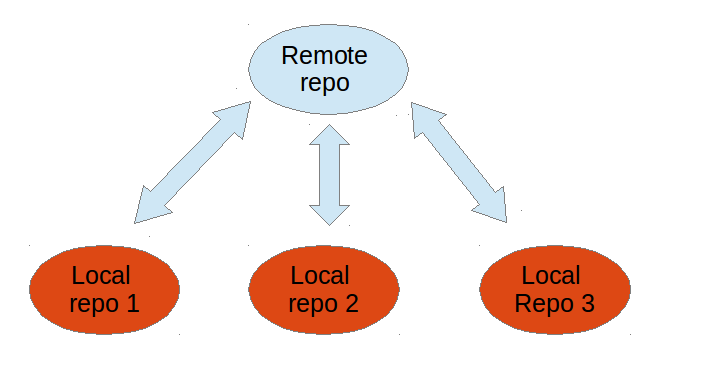
\includegraphics[angle=0,scale=0.5]{img/repo.png}
    \end{center}
    \caption{\em Schemat połączeń między repozytoriami Git}
    \label{fig:repo}
\end{figure}

Następnie zmiany mogą być wymieniane między lokalnymi repozytoriami. Służy do tego repozytorium zewnętrzne (remote repository) działające na serwerze. Serwisem przechowującym rozwijany projekt jest GitHub (\url{https://github.com/}), który udostępnia darmowy hosting open source. 


Repozytorium projektu jest dostępne pod adresem: \url{https://github.com/Gonz8/RSO-16L}

\section{Przygotowanie do pracy i pierwsze pobranie zawartości repozytorium}
	Na samym początku wymagane jest posiadanie klienta Git zainstalowanego w swoim systemie. Wszelkie istotne informacje dotyczące korzystania z Git możemy uzyskać wpisując w terminalu:
\begin{lstlisting}[style=incode]
$ git help
\end{lstlisting}
Następnie musimy określić własną nazwę oraz adres e-mail w systemie Git:
\begin{lstlisting}[style=incode]
$ git config --global user.name ''Your Name''
$ git config --global user.email ''address@example.com''
\end{lstlisting}
Aby zaimportować repozytorium ze wspomnianego serwera należy wykonać polecenie:
\begin{lstlisting}[style=incode]
$ git clone https://github.com/Gonz8/RSO-16L
\end{lstlisting}
Wszystkie pliki zostaną sklonowane do nowo utworzonego katalogu, z poziomu którego należy utworzyć lokalne repozytorium:
\begin{lstlisting}[style=incode]
$ git init
\end{lstlisting}
Utworzone w ten sposób repozytorium jest już powiązane ze zdalną wersją (origin). Możemy to sprawdzić przy użyciu polecenia:
\begin{lstlisting}[style=incode]
$ git remote -v
\end{lstlisting}

\section{Użytkowanie}

Po zaimportowaniu projektu oraz utworzeniu lokalnej kopii repozytorium można rozpocząć pracę z danymi. Aby sprawdzić status dokonanych zmian należy użyć w katalogu z kopią roboczą następującego polecenia:
\begin{lstlisting}[style=incode]
$ git status
\end{lstlisting}
Dodanie nowego pliku, kilku plików lub katalogu do kopii roboczej wykonywane jest przy użyciu komendy:
\begin{lstlisting}[style=incode]
$ git add <filename>
$ git add *
\end{lstlisting}
Aby zatwierdzić wszelkie dokonane zmiany w lokalnym repozytorium należy użyć polecenia:
\begin{lstlisting}[style=incode]
$ git commit -a
\end{lstlisting}
a następnie podać treść/opis poczynionych zmian.
W celu przechwycenia najnowszych zmian z serwera wykonujemy polecenie:
\begin{lstlisting}[style=incode]
$ git fetch origin
\end{lstlisting}
natomiast, aby przechwycić zmiany z serwera i dodatkowo dołączyć je do własnego katalogu roboczego wykonujemy polecenie:
\begin{lstlisting}[style=incode]
$ git pull
\end{lstlisting}

Wysłanie zmian poczynionych w wersji lokalnej do zdalnego repozytorium realizowane jest dzięki komendzie:
\begin{lstlisting}[style=incode]
$ git push origin master
$ git push origin <branchname>
\end{lstlisting}
Git pozwala również na tworzenie, usuwanie i przełączanie się między gałęziami projektu, do wykonania tych operacji służą następujące polecenia:
\begin{lstlisting}[style=incode]
$ git checkout -b <branchname>
$ git branch -d <branchname>
$ git checkout <branchname>
\end{lstlisting}
Wyświetlenie listy wszystkich gałęzi dostępnych w repozytorium możliwe jest poprzez komendę:
\begin{lstlisting}[style=incode]
$ git branch
\end{lstlisting}
Natomiast w celu dołączenia innej gałęzi do obecnie aktywnej należy wykonać polecenie:
\begin{lstlisting}[style=incode]
$ git merge <branchname>
\end{lstlisting}

Ostatnim również istotnym poleceniem jest wyświetlenie historii logów/commit'ów:
\begin{lstlisting}[style=incode]
$ git log
\end{lstlisting}

Dodatkowo po zainstalowaniu pakietu \textit{\textbf{gitk}} można wyświetlać graficzną prezentację historii zmian projektu.

\section{Dodatkowe narzędzia}
	Mimo faktu, że Git jest rozproszonym systemem kontroli wersji zdecydowano się na wykonywanie dodatkowej i okresowej kopii zapasowej projektu (tzw. backup). Kopia bezpieczeństwa jest jednym z elementów utrzymania repozytorium i zabezpiecza przed utratą danych (np. awarii może ulec komputer głównego programisty, przez co istnieje ryzyko utraty lokalnej kopii repozytorium) (...)

Serwis GitHub świadczy szereg dodatkowych usług wspomagających rozwój projektu programistycznego. Zdecydowano się wykorzystać usługę Wiki, gdzie w łatwy sposób można wprowadzać i modyfikować istotne treści w kontekście projektu. Jest to miejsce, gdzie można w szybki i wygodny sposób odnaleźć uporządkowane informacje. Jednym z odnośników w tej usłudze jest zakładka ''Dobre praktyki kodowania'', gdzie znajdują się wszystkie wspólnie ustalone przez programistów zasady pisania kodu pozwalające utrzymać przejrzystość i spójność kodu.

	Ponadto zdecydowano się uruchomić usługę śledzenia zgłoszeń (tzw. \textit{issue tracking}) na potrzeby wspierania testowania oprogramowania oraz zgłaszania napotkanych błędów i tworzenia dla nich poprawek.

\section{Przydatne informacje}
Instrukcja została opracowana na postawie materiałów znalezionych w sieci. Więcej informacji dotyczących użytkowania systemu kontroli wersji Git można znaleźć na stronach:
\begin{itemize}
\item \url{https://git-scm.com/docs/gittutorial}
\item \url{http://www.vogella.com/tutorials/Git/article.html\#git}
\end{itemize}